% !TEX root = ../../../main.tex

\toggletrue{image}
\toggletrue{imagehover}
\chapterimage{password_strength}
\chapterimagetitle{\uppercase{Password Strength}}
\chapterimageurl{https://xkcd.com/936/}
\chapterimagehover{\scriptsize To anyone who understands information theory and security and is in an infuriating argument with someone who does not (possibly involving mixed case), I sincerely apologize.}

\chapter{Polyalphabetische Kryptosysteme}
\label{chapter-polyalphabetische-kryptosysteme}

Wird ein Klartextbuchstabe nicht immer zum gleichen Kryptotextbuchstaben verschlüsselt, dann sind die Häufigkeiten der Klartextbuchstaben nicht mit den Häufigkeiten der Kryptotextbuchstaben identisch. Dieses Ziel verfolgen polyalphabetische Kryptosysteme. Die Lernziele lauten wie folgt:

\newcommand{\polyalphabetischeKryptosystemeLernziele}{
\protect\begin{todolist}
\item Sie erklären, was wir unter einem polyalphabetischen Kryptosystem verstehen.
\item Sie erklären jedes vorgestellte polyalphabetische Kryptosystem und wenden es an.
\item Sie führen die Kryptoanalyse für alle vorgestellten polyalphabetischen Kryptosysteme durch.
\end{todolist}
}

\lernziel{\autoref{chapter-polyalphabetische-kryptosysteme}, \nameref{chapter-polyalphabetische-kryptosysteme}}{\protect\polyalphabetischeKryptosystemeLernziele}

\polyalphabetischeKryptosystemeLernziele

\section{Was ist ein polyalphabetisches Kryptosystem?}

Polyalphabetische Kryptosysteme stellen den Gegensatz zu monoalphabetischen Systemen dar.

\begin{definition}
Ein Kryptosystem heisst \textbf{polyalphabetisch}, wenn \textbf{ein} Klartextbuchstabe für einen beliebigen, aber fixen Schlüssel zu \textbf{unterschiedlichen} Kryptotextbuchstaben verschlüsselt wird.
\end{definition}

\section{Das Kryptosystem \texttt{VIGENÈRE}}

Das berühmte Kryptosystem wurde im Jahre 1586 von Blaise de Vigenère veröffentlicht. Das Prinzip von \texttt{VIGENÈRE} (sprich Wischenähr) beruht darauf, dass sich verschiedene monoalphabetische Verschlüsselungen abwechseln. Das Klartext- und Kryptotextalphabet sind für das Kryptosystem \texttt{VIGENÈRE} identisch und beinhalten die \num{26} Grossbuchstaben (A bis Z).

\subsection{Schlüssel}

Sender und Empfänger müssen einen Schlüssel abmachen. Bei \texttt{VIGENÈRE} muss der Schlüssel ein \textbf{Wort über dem Klartextalphabet} sein. Der Schlüssel \textbf{muss} kein sinnvolles Wort darstellen.
 
 \begin{example}
Alice und Bob machen BAUM als Schlüssel ab.
 \end{example}

\subsection{Verschlüsselung und Entschlüsselung}

Für die \textbf{Verschlüsselung} notieren wir zunächst den Schlüssel \textbf{Buchstabe für Buchstabe} unter den Klartext (ohne Leerzeichen).  Falls der Klartext länger ist als der Schlüssel, dann wird der Schlüssel \textbf{wiederholt}. Falls der Schlüssel länger ist als der Klartext, dann wird der Schlüssel \say{abgeschnitten}.

\begin{example}
\label{encrypt-poly-1-example}
Wir notieren wiederholt den Schlüssel BAUM unter den Klartext.
\end{example}

\begin{table}[H]
\centering
\resizebox{\textwidth}{!}{%
\begin{tblr}{
    colspec = {|c|c|c|c|c|c|c|c|c|c|c|c|c|c|c|c|c|c|c|c|}
}
\hline
Klartext   & E & I & N & K & L & E & I & N & E & S & G & E & H & E & I & M & N & I & S \\ \hline
Schlüssel  & B & A & U & M & B & A & U & M & B & A & U & M & B & A & U & M & B & A & U \\ \hline
\end{tblr}
}
\end{table}

Für die eigentliche Verschlüsselung kommt dann das \textbf{Vigenère-Quadrat}  (\autoref{figure-vignere-quadrat-encrypt-example}) zum Einsatz. Das Vigenère-Quadrat ist öffentlich bekannt und bleibt immer gleich.

\begin{figure}[htb]
\centering
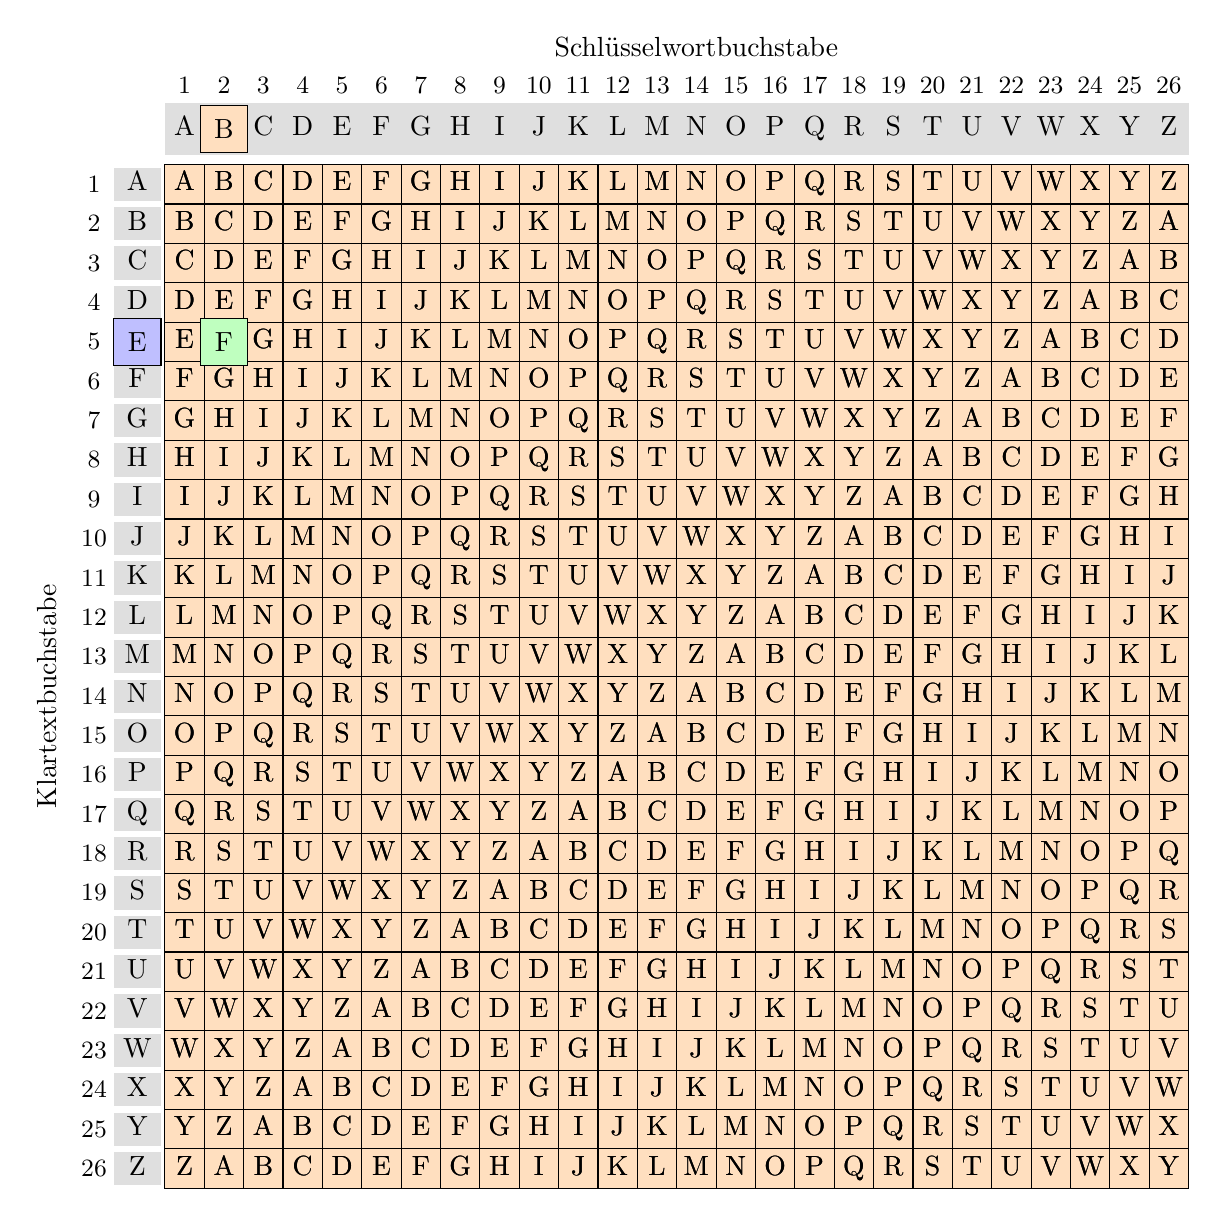
\begin{tikzpicture}
\foreach \i in {0,...,25} {
  \foreach \j in {0,...,25} {
    \edef\k{\ifnum\numexpr\i+\j\relax>25
        \the\numexpr\i+\j-26\relax
      \else
        \the\numexpr\i+\j\relax
      \fi}
 	\ifthenelse{\equal{\j}{4}} %E
 	{\node[draw, minimum size=0.5cm, inner sep=0pt, fill=blue!25] at (\i*0.5,-\j*0.5) {\strut\symbol{\numexpr`A+\k\relax}};}
 	{\node[draw, minimum size=0.5cm, inner sep=0pt] at (\i*0.5,-\j*0.5) {\strut\symbol{\numexpr`A+\k\relax}};}
	\ifthenelse{\equal{\i}{1}} %B
	{\node[draw, minimum size=0.5cm, inner sep=0pt, fill=orange!25] at (\i*0.5,-\j*0.5) {\strut\symbol{\numexpr`A+\k\relax}};}
 	{\node[draw, minimum size=0.5cm, inner sep=0pt] at (\i*0.5,-\j*0.5) {\strut\symbol{\numexpr`A+\k\relax}};}
  }
  \node[fill=gray!25, minimum width=0.6cm, inner sep=0pt, outer sep=0pt] at (-0.6,-\i*0.5) {\strut\symbol{\numexpr`A+\i\relax}};
  \node[minimum width=0.6cm] at (-1.15,-\i*0.5) {\small \the\numexpr\i+1};
  
  \node[fill=gray!25, minimum width=0.5cm] at (\i*0.5,0.7)   {\strut\symbol{\numexpr`A+\i\relax}};
  \node[minimum width=0.5cm] at (\i*0.5,1.25) {\small \the\numexpr\i+1};
}

\node[draw, minimum size=0.6cm, fill=orange!25]
    at (1*0.5, 0.7) {B};
\node[draw, minimum size=0.6cm, fill=blue!25]
    at (-0.6, -4*0.5) {E};
\node[draw, minimum size=0.6cm, fill=green!25]
    at (1*0.5, -4*0.5) {F};

\node[rotate=90, anchor=north] at (-2,-6.5) {Klartextbuchstabe};
\node at (6.5,1.75) {Schlüsselwortbuchstabe};
\end{tikzpicture}
\caption{Beispiel einer Verschlüsselung: E mit B wird zu F verschlüsselt.}
\label{figure-vignere-quadrat-encrypt-example}
\end{figure}

Der Klartext wird Buchstabe für Buchstabe verschlüsselt. Der Klartextbuchstabe bestimmt die \textbf{Zeile}, der darunter liegende Schlüsselwortbuchstabe die \textbf{Spalte} im Vigenère-Quadrat. Den Kryptotextbuchstaben erhalten wir durch den \textbf{Schnittpunkt} von Zeile und Spalte.

\begin{example}
\label{encrypt-poly-2-example}
Wir setzen \autoref{encrypt-poly-1-example} fort. Der erste Klartextbuchstabe lautet E. Unter dem E steht der Schlüsselwortbuchstabe B. Die Zeile mit dem E (blaue Zeile) kreuzt sich mit der B-Spalte (orange Spalte) in der Zelle mit dem F. Somit wird der Buchstabe E mit B zu F verschlüsselt. Diesen Vorgang wiederholen wir für jeden weiteren Klartextbuchstaben.
\end{example}

\begin{table}[H]
\centering
\resizebox{\textwidth}{!}{%
\begin{tblr}{
    colspec = {|c|c|c|c|c|c|c|c|c|c|c|c|c|c|c|c|c|c|c|c|},
    cell{1}{2} = {blue!25},
    cell{2}{2} = {orange!25},
    cell{3}{2} = {green!25}
}
\hline
Klartext   & E & I & N & K & L & E & I & N & E & S & G & E & H & E & I & M & N & I & S \\ \hline
Schlüssel  & B & A & U & M & B & A & U & M & B & A & U & M & B & A & U & M & B & A & U \\ \hline[2pt]
Kryptotext  & F & I & H & W & M & E & C & Z & F & S & A & Q & I & E & C & Y & O & I & M \\ \hline
\end{tblr}
}
\end{table}

Die \textbf{Entschlüsselung} läuft sehr ähnlich. Wir schreiben dieses Mal den \textbf{Kryptotext unter den Schlüssel}. Dann suchen wir im Vigenère-Quadrat den Schlüsselwortbuchstaben in der \textbf{grauen Zeile}. In dieser \textbf{Spalte} suchen wir den \textbf{Kryptotextbuchstaben}. Den Klartextbuchstaben lesen wir jetzt \textbf{ganz links} in der \textbf{grauen Spalte} ab.

\begin{example}
Wir entschlüsseln den Kryptotext QALFZIHPFREEXEGQOSU mit dem gleichen Schlüssel BAUM. Unter dem Schlüsselwortbuchstaben U steht der Kryptotextbuchstabe L. Wir suchen in der Spalte mit dem U (orange Spalte) den Kryptotextbuchstaben L (grüne Zelle). Danach lesen wir ganz links (blaue Zeile) den Klartextbuchstaben R ab. Somit wird der Buchstabe L mit U zu R entschlüsselt. Diesen Vorgang wiederholen wir für jeden anderen Kryptotextbuchstaben.
\end{example}

\begin{table}[H]
\centering
\resizebox{\textwidth}{!}{%
\begin{tblr}{
    colspec = {|c|c|c|c|c|c|c|c|c|c|c|c|c|c|c|c|c|c|c|c|},
    cell{1}{4} = {orange!25},
    cell{2}{4} = {green!25},
    cell{3}{4} = {blue!25}
}
\hline
Schlüssel  & B & A & U & M & B & A & U & M & B & A & U & M & B & A & U & M & B & A & U \\ \hline
Kryptotext  & Q & A & L & F & Z & I & H & P & F & R & E & E & X & E & G & Q & O & S & U \\ \hline[2pt]
Klartext   & P & A & R & T & Y & I & N & D & E & R & K & S & W & E & M & E & N & S & A \\ \hline
\end{tblr}
}
\end{table}

\begin{figure}[htb]
\centering
\begin{tikzpicture}
\foreach \i in {0,...,25} {
  \foreach \j in {0,...,25} {
    \edef\k{\ifnum\numexpr\i+\j\relax>25
        \the\numexpr\i+\j-26\relax
      \else
        \the\numexpr\i+\j\relax
      \fi}
 	\ifthenelse{\j = 17 \and \i < 21} %R
 	{\node[draw, minimum size=0.5cm, inner sep=0pt, fill=blue!25] at (\i*0.5,-\j*0.5) {\strut\symbol{\numexpr`A+\k\relax}};}
 	{\node[draw, minimum size=0.5cm, inner sep=0pt] at (\i*0.5,-\j*0.5) {\strut\symbol{\numexpr`A+\k\relax}};}
	\ifthenelse{\equal{\i}{20}} %U
	{\node[draw, minimum size=0.5cm, inner sep=0pt, fill=orange!25] at (\i*0.5,-\j*0.5) {\strut\symbol{\numexpr`A+\k\relax}};}
 	{\node[draw, minimum size=0.5cm, inner sep=0pt] at (\i*0.5,-\j*0.5) {\strut\symbol{\numexpr`A+\k\relax}};}
  }
  \node[fill=gray!25, minimum width=0.6cm, inner sep=0pt, outer sep=0pt] at (-0.6,-\i*0.5) {\strut\symbol{\numexpr`A+\i\relax}};
  \node[minimum width=0.6cm] at (-1.15,-\i*0.5) {\small \the\numexpr\i+1};
  
  \node[fill=gray!25, minimum width=0.5cm] at (\i*0.5,0.7)   {\strut\symbol{\numexpr`A+\i\relax}};
  \node[minimum width=0.5cm] at (\i*0.5,1.25) {\small \the\numexpr\i+1};
}

\node[draw, minimum size=0.6cm, fill=orange!25]
    at (20*0.5, 0.7) {U};
\node[draw, minimum size=0.6cm, fill=blue!25]
    at (-0.6, -17*0.5) {R};
\node[draw, minimum size=0.6cm, fill=green!25]
    at (20*0.5, -17*0.5) {L};

\node[rotate=90, anchor=north] at (-2,-6.5) {Klartextbuchstabe};
\node at (6.5,1.75) {Schlüsselwortbuchstabe};
\end{tikzpicture}
\caption{Beispiel einer Entschlüsselung: L mit U wird zu R entschlüsselt.}
\label{figure-vignere-quadrat-decrypt-example}
\end{figure}

\subsection{Schlüsselmenge}

Die Grösse der Schlüsselmenge, das heisst $|\mathscr{S}_{\texttt{VIGENÈRE}}|$, hängt von der \textbf{Länge des Schlüsselworts} ab. Besitzt das Schlüsselwort $n$ Buchstaben, dann gilt $|\mathscr{S}_{\texttt{VIGENÈRE}}| = 26^n$.

\subsection{Polyalphabetisch?}

Bei \texttt{VIGENÈRE} gleichen sich die Häufigkeiten der einzelnen Buchstaben aus, da ein Klartextbuchstabe auf verschiedene Kryptotextbuchstaben abgebildet wird. Der Klartextbuchstabe N aus \autoref{encrypt-poly-2-example} wird zu drei unterschiedlichen Kryptotextbuchstaben verschlüsselt (siehe \autoref{figure-vigenere-poly}).

\begin{figure}[htb]
\centering
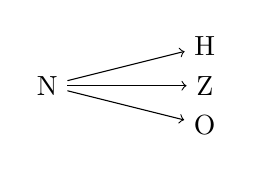
\begin{tikzpicture}
\node (N) at (0,0) {N};
\node (H) at (2,0.5) {H};
\node (Z) at (2,0) {Z};
\node (O) at (2,-0.5) {O};
\draw[->] (N) -- (H);
\draw[->] (N) -- (Z);
\draw[->] (N) -- (O);
\end{tikzpicture}
\caption{Das N wird in \autoref{encrypt-poly-2-example} zu H, Z und O verschlüsselt.}
\label{figure-vigenere-poly}
\end{figure}

\vspace{-0.25cm}

Die polyalphabetische Eigenschaft entsteht dadurch, in dem die Kombination aus Klartext- und Schlüsselwortbuchstabe den Kryptotextbuchstaben bestimmt.

\subsection{Kryptoanalyse}

Bereits 1863 gelang das Knacken eines Kryptotextes. Friedrich Wilhelm Kasiski hatte eine Methode entwickelt, um die Schlüsselwortlänge einzugrenzen. Auch William Frederick Friedman erarbeitete \num{70} Jahre nach Kasiski eine Methode, um \texttt{VIGENÈRE} effizienter zu knacken. Wir präsentieren hier nun den Kasiski-Test (ein Angriff mit bekanntem Kryptotext).

\subsubsection{1. Schritt des Kasiski-Tests: Schlüssellänge bestimmen}

Wie gehen wir nun vor, um \texttt{VIGENÈRE} zu knacken? Schauen wir folgenden Kryptotext an:

\begin{table}[htb]
\ttfamily
\SetTblrInner{colsep=1pt}
\centering
\begin{tblr}{
    colspec = {ccccc},
    cell{1}{1} = {orange!25},
    cell{1}{2} = {magenta!25},
    cell{1}{3} = {orange!25},
    cell{1}{5} = {magenta!25}
}
NEQ & SWR & NEQ & DSPSRBOQBOVQMLJEIQCIJ & SWR
\end{tblr}
\end{table}

\vspace{-0.25cm}

Der Kryptotext wurde mit dem Schlüssel KEY verschlüsselt. Wir können im Kryptotext erkennen, dass sich die Kryptotextwörter NEQ und SWR \textbf{wiederholen}. Die Wiederholung ist dadurch entstanden, dass die Klartextwörter DAS bzw. IST jeweils zweimal mit den gleichen Schlüsselwortbuchstaben verschlüsselt wurden (\autoref{table-vigenere-kryptoanalyse-1}).

\vspace{-0.25cm}

\begin{table}[htb]
\ttfamily
\SetTblrInner{colsep=1pt}
\centering
\begin{tblr}{
    colspec = {p{2cm}lllll},
    cell{1}{2} = {orange!25},
    cell{1}{3} = {magenta!25},
    cell{1}{4} = {orange!25},
    cell{1}{6} = {magenta!25},
    cell{2}{2} = {orange!25},
    cell{2}{3} = {magenta!25},
    cell{2}{4} = {orange!25},
    cell{2}{6} = {magenta!25},
    cell{3}{2} = {orange!25},
    cell{3}{3} = {magenta!25},
    cell{3}{4} = {orange!25},
    cell{3}{6} = {magenta!25}
}
\textrm{Klartext:}	& DAS & IST & DAS & TORINDEMDERSCHLUESSEL & IST \\ 
\textrm{Schlüssel:} 	& KEY & KEY & KEY & KEYKEYKEYKEYKEYKEYKEY & KEY \\
\textrm{Kryptotext:}	& NEQ & SWR & NEQ & DSPSRBOQBOVQMLJEIQCIJ & SWR
\end{tblr}
\caption{Folgen von Klartextbuchstaben fallen auf die gleichen Schlüsselwortbuchstaben.}
\label{table-vigenere-kryptoanalyse-1}
\end{table}

\vspace{-0.25cm}

Mit dieser Erkenntnis erfahren wir etwas über die \textbf{Schlüssellänge}. Wir tun nun einmal so, als wüssten wir den Schlüssel nicht. Dann betrachten wir den Abstand zwischen den Anfangsbuchstaben.

\begin{table}[H]
\ttfamily
\centering
\begin{tblr}{
    colspec = {p{1.75cm}ccccccccclccc},
    cell{1}{2} = {orange!25},
    cell{1}{8} = {orange!25},
    cell{1}{5} = {magenta!25},
    cell{1}{12} = {magenta!25}
}
\textrm{Kryptotext:} 				& N 	& E 	& Q 	& S &W & R & N & E & Q & DSPSRBOQBOVQMLJEIQCIJ & S & W & R \\
\textrm{Position:} 				& 1 	& 2 	& 3 	& 4 & 5 & 6 & 7 & 8 & 9 & 10 $\cdots$ $\cdots$ $\cdots$ $\cdots$ $\cdots$ 30 & 31 & 32 & 33 \\
\SetCell[r=2]{l}{\textrm{Abstand:}} 	& \SetCell[c=7]{c}{$\xrightarrow{\makebox[3.5cm]{$+6$}}$} & & & & & & & & & & & & \\
							& 	& 	& 	& \SetCell[c=8]{c}{$\xrightarrow{\makebox[8.5cm]{$+27$}}$} & 32 & 33
\end{tblr}
\end{table}


Zwischen dem ersten und zweiten Auftreten des Kryptotextwortes NEQ liegen \num{6} Kryptotextbuchstaben. Zwischen den beiden Kryptotextworten SWR liegen \num{27} Kryptotextbuchstaben. Beide Zahlen sind ein Vielfaches von \num{3} (= Schlüssellänge). Wir können diesen Sachverhalt verallgemeinern. Wenn das gleiche Kryptotextwort an zwei verschiedenen Positionen auftritt, dann muss die Differenz zwischen den beiden Positionen entweder genau der Schlüssellänge entsprechen oder ein Vielfaches der Schlüssellänge sein. Somit muss die Schlüssellänge ein \textbf{Teiler der Differenz} der beiden Positionen sein.

\begin{important}[Mögliche Schlüssellänge bestimmen]
Anleitung zur Kryptoanalyse:
\begin{enumerate}
\item Wir identifizieren möglichst alle Kryptotextwörter, die sich wiederholen.
\item Positionen der Wiederholungen bestimmen.
\item Differenzen zwischen je zwei Positionen bilden.
\item \acs{ggT} der Differenzen berechnen.
\end{enumerate}
Entweder entspricht der \acs{ggT} der Schlüssellänge oder es ist ein Teiler des \acs{ggT}s.
\end{important}

Wir bestimmen den \ac{ggT} mit der Primfaktorzerlegung der Differenzen oder mit dem Algorithmus von Euklid. Wir zeigen das Vorgehen nun an zwei Beispielen. Wir verzichten auf die \say{manuelle} Berechnung des \ac{ggT}s und verwenden ein Hilfsmittel (Taschenrechner, Computerprogramm etc.). 

\begin{example}
Im Kryptotext NEQSWRNEQDSPSRBOQBOVQMLJEIQCIJSWR wiederholen sich die Wörter NEQ und SWR. \autoref{table-neq-swr} zeigt die Positionen und die Differenzen.

\begin{table}[htb]
\centering
\begin{tblr}{
    colspec = {|c|c|c|c|}
}
\hline
Kryptotextwort & 1. Position & 2. Position & Differenz   \\ \hline
NEQ            & $1$           & $7$           & $7 - 1 = 6$   \\ \hline
SWR            & $4$           & $31$          & $31 - 4 = 27$ \\ \hline
\end{tblr}
\caption{Die Position wird mithilfe des 1. Buchstabens bestimmt.}
\label{table-neq-swr}
\end{table}

Der \ac{ggT} von \num{6} und \num{27} lautet \num{3}. Für die Schlüssellänge kommt somit \num{3} oder ein Teiler von \num{3} infrage. Da \num{1} der einzige Teiler ist, gehen wir davon aus, dass der Schlüssel eine Länge von \num{3} hat (was wir ja bereits wissen, da der Schlüssel in diesem Beispiel KEY lautet).
\end{example}

\begin{example}
\label{example-break-vigenere-2-schluessellaenge}
Der Kryptotext VRGRHF\colorbox{orange!30}{VIG}VBBINX\colorbox{orange!30}{VIG}VNTGFXCUGU\colorbox{magenta!30}{EBEE}URNTEENE DUVEGUEMVDTDIMJ\colorbox{magenta!30}{EBEE}G\colorbox{orange!30}{VIG}BANW beinhaltet EBEE und VIG mehrmals.

\begin{table}[htb]
\centering
\begin{tblr}{
    colspec = {|c|c|c|c|c|}
}
\hline
Kryptotextwort & 1. Pos. & 2. Pos. & 3. Pos. & Differenzen   \\ \hline
VIG            & $7$           & $16$    & $61$        & {$16 - 7 = 9$ \\ $61 - 16 = 45$ \\ $61 - 7 = 54$}   \\ \hline
EBEE            & $29$           & $56$          & & $56 - 29 = 27$ \\ \hline
\end{tblr}
\caption{Bei mehr als zwei Positionen müssen alle Differenzen ausgerechnet werden.}
\label{table-vig-ebee}
\end{table}

Für den \ac{ggT} von \num{9}, \num{45}, \num{54} und \num{27} erhalten wir \num{9}. Wir schreiben dafür $ggT(9, 27, 45, 54) = 9$. Für die Schlüssellänge kommen somit \num{9} und \num{3} infrage.
\end{example}

In \autoref{example-break-vigenere-2-schluessellaenge} sind beide Schlüssellängen plausibel. Wir müssten den zweiten Schritt des  Kasiski-Tests eventuell für beide Schlüssellängen durchführen. Als Alternative können wir den Friedman-Test durchführen.

\begin{important}[Friedman-Test]
Bei diesem Test erhalten wir eine grobe (!) Einschätzung für die Schlüsselwortlänge. Für den Kryptotext aus \autoref{example-break-vigenere-2-schluessellaenge} erhalten wir mit dem Friedman-Test eine Schlüssellänge von \num{1,069}. Diese Zahl liegt näher bei der Schlüsselwortlänge \num{3} statt \num{9}. Es liegt nun nahe, den nächsten Schritt des Kasiski-Tests für den Kryptotext aus \autoref{example-break-vigenere-2-schluessellaenge} mit der Schlüsselwortlänge \num{3} durchzuführen.
\end{important}

\newpage

\subsubsection{2. Schritt des Kasiski-Tests: Schlüsselwortbuchstaben bestimmen}

Obwohl es bei einer Schlüssellänge von $n$ Buchstaben immer noch $26^n$ verschiedene Schlüssel gibt, ist es nun einfacher den Kryptotext zu analysieren. Wir zeigen nun, wie wir dazu vorgehen. Wir verwenden dazu einen anderen Kryptotext, bei dem wir bereits vermuten, dass die Schlüssellänge \num{5} ist. Deshalb haben wir den Kryptotext in Blöcke der Länge \num{5} eingeteilt.\\

\begin{example}
Folgender Kryptotext wurde mit einem Schlüsselwort der Länge \num{5} erstellt.
\label{example-kryptotext-kasiski-2}
%DQRSEMVOUQLBETIHVISFQCRTIMQROVKIRJZNZFKMDZWIL
%ZCXNMMCRZIQCRJYDJIXPDOXCMDBMKJDALOIQESNPHAXJE
%DZRAVDQRYGGEEXDDAPUGGAMKLSPIHXDZIORDVORIHVITW
%SMMTETNYTHVQVLXHPRNMMMMTYMLIXPZCWILSTEAWBPXRE
%TAGNXGWIXXZJIXODQRKRZCJVVZTPGPRWYKFDZPKKSMVYM
%BPHGWRMVCSGTIORDVKXSDAWKVDVWZIHVFXETKLZKDAEMX
%FMXGRDZJORCMXKMMMVOIRMRMVNAWKRRBIORGMFZMGVQOX
%KMXFXDZOXEEBLUGGCRJAHZJZMGVMTHDVFXYMVITAZMLXI
%MLIXRNKLGYELITETNTXEKTAGVSMXYMDPXKVZCJKMMUERI
%HVIFMDOIJMDQRKMMMQGJEMRFEGVEAJHPRFYQMRTXTVHOR
%CMRHVTVRKRRXVORFBIXHDVOZWHKLSIMAGNMBHGWQIXI
%HVWKPSAESIRTETHVWFORHKLJIMVHGKDTETHDBRGGGMMTI
%QEIOPDSSSQSMMTDVMMZIQUETRTVHLVZOXNERBHAQDQRKD
%HMKKKDAINIMMVGRSESXXDBMILVMMYWIIROGGBSHIRLIOR
%DEEXHZAAGVDQRYIKBWGQDAZOIBPHOIHAXJSBPIILSMMTJ
%ZKLORCMRHVTVRKRFMWVVTVKKRCIVGYEUIORSLIXQZVRTI
%HVQKMMMOGRMLEYRHKLZKDEIYIMAIORCQINEAQGNEMMMTI
%LAXKMMNIYXFMFARCMR

\scriptsize
\texttt{\colorbox{orange!30}{D}QRSE\colorbox{orange!30}{M}VOUQ\colorbox{orange!30}{L}BETI\colorbox{orange!30}{H}VISF\colorbox{orange!30}{Q}CRTI\colorbox{orange!30}{M}QROV\colorbox{orange!30}{K}IRJZ\colorbox{orange!30}{N}ZFKM\colorbox{orange!30}{D}ZWIL\colorbox{orange!30}{Z}CXNM\colorbox{orange!30}{M}CRZI\colorbox{orange!30}{Q}CRJY\colorbox{orange!30}{D}JIXP\colorbox{orange!30}{D}OXCM\colorbox{orange!30}{D}BMKJ\colorbox{orange!30}{D}ALOI\\
\colorbox{orange!30}{Q}ESNP\colorbox{orange!30}{H}AXJE\colorbox{orange!30}{D}ZRAV\colorbox{orange!30}{D}QRYG\colorbox{orange!30}{G}EEXD\colorbox{orange!30}{D}APUG\colorbox{orange!30}{G}AMKL\colorbox{orange!30}{S}PIHX\colorbox{orange!30}{D}ZIOR\colorbox{orange!30}{D}VORI\colorbox{orange!30}{H}VITW\colorbox{orange!30}{S}MMTE\colorbox{orange!30}{T}NYTH\colorbox{orange!30}{V}QVLX\colorbox{orange!30}{H}PRNM\colorbox{orange!30}{M}MMTY\\
\colorbox{orange!30}{M}LIXP\colorbox{orange!30}{Z}CWIL\colorbox{orange!30}{S}TEAW\colorbox{orange!30}{B}PXRE\colorbox{orange!30}{T}AGNX\colorbox{orange!30}{G}WIXX\colorbox{orange!30}{Z}JIXO\colorbox{orange!30}{D}QRKR\colorbox{orange!30}{Z}CJVV\colorbox{orange!30}{Z}TPGP\colorbox{orange!30}{R}WYKF\colorbox{orange!30}{D}ZPKK\colorbox{orange!30}{S}MVYM\colorbox{orange!30}{B}PHGW\colorbox{orange!30}{R}MVCS\colorbox{orange!30}{G}TIOR\\
\colorbox{orange!30}{D}VKXS\colorbox{orange!30}{D}AWKV\colorbox{orange!30}{D}VWZI\colorbox{orange!30}{H}VFXE\colorbox{orange!30}{T}KLZK\colorbox{orange!30}{D}AEMX\colorbox{orange!30}{F}MXGR\colorbox{orange!30}{D}ZJOR\colorbox{orange!30}{C}MXKM\colorbox{orange!30}{M}MVOI\colorbox{orange!30}{R}MRMV\colorbox{orange!30}{N}AWKR\colorbox{orange!30}{R}BIOR\colorbox{orange!30}{G}MFZM\colorbox{orange!30}{G}VQOX\colorbox{orange!30}{K}MXFX\\
\colorbox{orange!30}{D}ZOXE\colorbox{orange!30}{E}BLUG\colorbox{orange!30}{G}CRJA\colorbox{orange!30}{H}ZJZM\colorbox{orange!30}{G}VMTH\colorbox{orange!30}{D}VFXY\colorbox{orange!30}{M}VITA\colorbox{orange!30}{Z}MLXI\colorbox{orange!30}{M}LIXR\colorbox{orange!30}{N}KLGY\colorbox{orange!30}{E}LITE\colorbox{orange!30}{T}NTXE\colorbox{orange!30}{K}TAGV\colorbox{orange!30}{S}MXYM\colorbox{orange!30}{D}PXKV\colorbox{orange!30}{Z}CJKM\\
\colorbox{orange!30}{M}UERI\colorbox{orange!30}{H}VIFM\colorbox{orange!30}{D}OIJM\colorbox{orange!30}{D}QRKM\colorbox{orange!30}{M}MQGJ\colorbox{orange!30}{E}MRFE\colorbox{orange!30}{G}VEAJ\colorbox{orange!30}{H}PRFY\colorbox{orange!30}{Q}MRTX\colorbox{orange!30}{T}VHOR\colorbox{orange!30}{C}MRHV\colorbox{orange!30}{T}VRKR\colorbox{orange!30}{R}XVOR\colorbox{orange!30}{F}BIXH\colorbox{orange!30}{D}VOZW\colorbox{orange!30}{H}KLSI\\
\colorbox{orange!30}{M}AGNM\colorbox{orange!30}{R}BHGW\colorbox{orange!30}{G}QIXI\colorbox{orange!30}{H}VWKP\colorbox{orange!30}{S}AESI\colorbox{orange!30}{R}TETH\colorbox{orange!30}{V}WFOR\colorbox{orange!30}{H}KLJI\colorbox{orange!30}{M}VHGK\colorbox{orange!30}{D}TETH\colorbox{orange!30}{D}BRGG\colorbox{orange!30}{G}MMTI\colorbox{orange!30}{Q}EIOP\colorbox{orange!30}{D}SSSQ\colorbox{orange!30}{S}MMTD\colorbox{orange!30}{V}MMZI\\
\colorbox{orange!30}{Q}UETR\colorbox{orange!30}{T}VHLV\colorbox{orange!30}{Z}OXNE\colorbox{orange!30}{R}BHAQ\colorbox{orange!30}{D}QRKD\colorbox{orange!30}{H}MKKK\colorbox{orange!30}{D}AINI\colorbox{orange!30}{M}MVGR\colorbox{orange!30}{S}ESXX\colorbox{orange!30}{D}BMIL\colorbox{orange!30}{V}MMYW\colorbox{orange!30}{I}IROG\colorbox{orange!30}{G}BSHI\colorbox{orange!30}{R}LIOR\colorbox{orange!30}{D}EEXH\colorbox{orange!30}{Z}AAGV\\
\colorbox{orange!30}{D}QRYI\colorbox{orange!30}{K}BWGQ\colorbox{orange!30}{D}AZOI\colorbox{orange!30}{B}PHOI\colorbox{orange!30}{H}AXJS\colorbox{orange!30}{B}PIIL\colorbox{orange!30}{S}MMTJ\colorbox{orange!30}{Z}KLOR\colorbox{orange!30}{C}MRHV\colorbox{orange!30}{T}VRKR\colorbox{orange!30}{F}MWVV\colorbox{orange!30}{T}VKKR\colorbox{orange!30}{C}IVGY\colorbox{orange!30}{E}UIOR\colorbox{orange!30}{S}LIXQ\colorbox{orange!30}{Z}VRTI\\
\colorbox{orange!30}{H}VQKM\colorbox{orange!30}{M}MOGR\colorbox{orange!30}{M}LEYR\colorbox{orange!30}{H}KLZK\colorbox{orange!30}{D}EIYI\colorbox{orange!30}{M}AIOR\colorbox{orange!30}{C}QINE\colorbox{orange!30}{A}QGNE\colorbox{orange!30}{M}MMTI\colorbox{orange!30}{L}AXKM\colorbox{orange!30}{M}NIYX\colorbox{orange!30}{F}MFAR\colorbox{orange!30}{C}MR
}\\

\end{example}


\normalsize

Wir können nun die Kryptotextbuchstaben in $5$ Gruppen einteilen. Jede Gruppe steht für einen (noch) unbekannten Schlüsselbuchstaben. Im Kryptotext sind alle Buchstaben markiert, welche mit dem ersten Buchstaben des Schlüssels ($s_1$) verschlüsselt wurden (siehe \autoref{table-s1}). 

\begin{table}[htb]
\centering
\begin{tabular}{|c|p{13cm}|}
\hline
\footnotesize Gruppe & \footnotesize Kryptotextbuchstaben                                                                                                                                                                                                                                                                                                         \\ \hline
\footnotesize s\_1   & \footnotesize D M L H Q M K N D Z M Q D D D D Q H D D G D G S D D H S T V H M M Z S B T G Z D Z Z R D S B R G D D D H T D F D C M R N R G G K D E G H G D M Z M N E T K S D Z M H D D M E G H Q T C T R F D H M R G H S R V H M D D G Q D S V Q T Z R D H D M S D V I G R D Z D K D B H B S Z C T F T C E S Z H M M H D M C A M L M F C \\ \hline
\end{tabular}
\caption{Die erste von fünf Gruppen.}
\label{table-s1}
\end{table}

Wir wissen nicht, welcher Schlüsselbuchstabe benutzt wurde, jedoch wurden \textbf{alle} Buchstaben aus $s_1$ identisch verschlüsselt. Wir müssen also die \textbf{Schlüsselwortspalte} im \textbf{Vigenère-Quadrat} ermitteln. 

\begin{important}
In jeder Schlüsselwortspalte im Vigenère-Quadrat ist das Alphabet vertikal \say{verschoben}. Es handelt sich somit um eine einfache \texttt{CAESAR}-Verschlüsselung.
\end{important}

Wir wissen nun, dass die Kryptotextbuchstaben aus der Gruppe $s_1$ einer \textbf{monoalphabetischen Verschlüsselung} unterliegen. Wir können wieder die Häufigkeitsanalyse anwenden, um den Schlüsselbuchstaben $s_1$ herauszufinden. Dazu zählen wir die Buchstaben in der Gruppe $s_1$. Das Häufigkeitsdiagramm aus \autoref{figure-haufigkeitsdiagramm_s1-1} zeigt, dass der Kryptotextbuchstabe D am häufigsten in der Gruppe $s_1$ vorkommt.

\begin{figure}[htb]
\centering
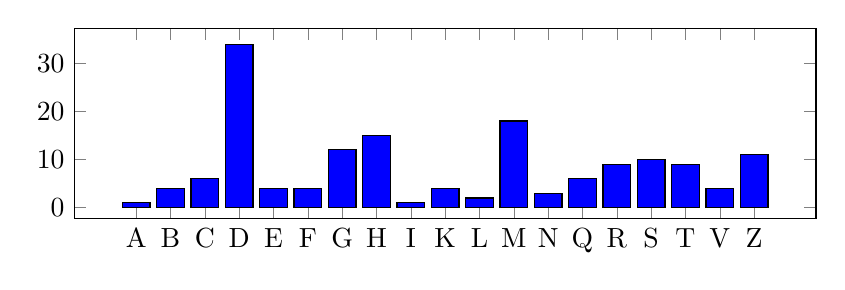
\begin{tikzpicture}
\begin{axis}[
symbolic x coords={
A, B, C, D, E, F, G, H, I, K, L, M, N, Q, R, S, T, V, Z
}, xtick=data, height=4cm, width=11cm
]
\addplot[ybar, fill=blue] coordinates {
(A, 1)
(B, 4)
(C, 6)
(D, 34)
(E, 4)
(F, 4)
(G, 12)
(H, 15)
(I, 1)
(K, 4)
(L, 2)
(M, 18)
(N, 3)
(Q, 6)
(R, 9)
(S, 10)
(T, 9)
(V, 4)
(Z, 11)
};
\end{axis}
\end{tikzpicture}
\caption{Häufigkeitsdiagramm für die Kryptotextbuchstaben aus der Gruppe $s_1$.}
\label{figure-haufigkeitsdiagramm_s1-1}
\end{figure}

Gehen wir davon aus, dass es sich beim Klartext um einen Text in deutscher Sprache handelt, dann ist der häufigste Buchstabe ein E. Somit liegt die Vermutung nahe, dass der \textbf{Kryptotextbuchstabe D durch die Verschlüsselung des Buchstabens E} entstanden ist. 

\newpage

Wir können somit im Vigenère-Quadrat nach dem Schlüsselwortbuchstaben suchen, welcher den Buchstaben E (blaue Zeile) zu einem D (grüne Zelle) verschlüsselt. Dies ist der Buchstabe Z (orange Spalte). In \autoref{figure-vignere-quadrat-kryptoanalyse} ist der Suchvorgang farblich markiert.

\begin{figure}[htb]
\centering
\begin{tikzpicture}
\foreach \i in {0,...,25} {
  \foreach \j in {0,...,25} {
    \edef\k{\ifnum\numexpr\i+\j\relax>25
        \the\numexpr\i+\j-26\relax
      \else
        \the\numexpr\i+\j\relax
      \fi}
 	\ifthenelse{\j = 4 \and \i < 26} %E
 	{\node[draw, minimum size=0.5cm, inner sep=0pt, fill=blue!25] at (\i*0.5,-\j*0.5) {\strut\symbol{\numexpr`A+\k\relax}};}
 	{\node[draw, minimum size=0.5cm, inner sep=0pt] at (\i*0.5,-\j*0.5) {\strut\symbol{\numexpr`A+\k\relax}};}
	\ifthenelse{\j < 4 \and \i = 25} %U
	{\node[draw, minimum size=0.5cm, inner sep=0pt, fill=orange!25] at (\i*0.5,-\j*0.5) {\strut\symbol{\numexpr`A+\k\relax}};}
 	{\node[draw, minimum size=0.5cm, inner sep=0pt] at (\i*0.5,-\j*0.5) {\strut\symbol{\numexpr`A+\k\relax}};}
  }
  \node[fill=gray!25, minimum width=0.6cm, inner sep=0pt, outer sep=0pt] at (-0.6,-\i*0.5) {\strut\symbol{\numexpr`A+\i\relax}};
  \node[minimum width=0.6cm] at (-1.15,-\i*0.5) {\small \the\numexpr\i+1};
  
  \node[fill=gray!25, minimum width=0.5cm] at (\i*0.5,0.7)   {\strut\symbol{\numexpr`A+\i\relax}};
  \node[minimum width=0.5cm] at (\i*0.5,1.25) {\small \the\numexpr\i+1};
}

\node[draw, minimum size=0.6cm, fill=orange!25]
    at (25*0.5, 0.7) {Z};
\node[draw, minimum size=0.6cm, fill=blue!25]
    at (-0.6, -4*0.5) {E};
\node[draw, minimum size=0.6cm, fill=green!25]
    at (25*0.5, -4*0.5) {D};

\node[rotate=90, anchor=north] at (-2,-6.5) {Klartextbuchstabe};
\node at (6.5,1.75) {Schlüsselwortbuchstabe};
\end{tikzpicture}
\caption{Alle Kryptotextbuchstaben der Gruppe $s_1$ wurden vermutlich mit Z verschlüsselt.}
\label{figure-vignere-quadrat-kryptoanalyse}
\end{figure}

\vspace{-0.25cm}

Daraus können wir nun schliessen, dass es sich bei den Kryptotextbuchstaben aus $s_1$ um eine \texttt{CAESAR}-Verschlüsselung mit einer Verschiebung um $25$ Positionen handelt. Wir können somit für die Gruppe $s_1$ die Verschlüsselung für jeden Klartextbuchstaben bestimmen (siehe \autoref{table-caesar-25}).

\vspace{-0.25cm}

\begin{table}[H]
\centering
\begin{tblr}{
    colspec = {|c|c|c|c|c|c|c|c|c|c|c|c|c|c|c|c|c|c|c|c|c|c|c|c|c|c|c|}
}
\hline
Klartextbuchstabe 	& A & B & C & D & E & F & G & H & I & J & K & L & M \\ \hline
Kryptotextbuchstabe & Z & A & B & C & D & E & F & G & H & I & J & K & L  \\ \hline[2pt]
Klartextbuchstabe & N & O & P & Q & R & S & T & U & V & W & X & Y & Z \\ \hline
Kryptotextbuchstabe & M & N & O & P & Q & R & S & T & U & V & W & X & Y  \\ \hline
\end{tblr}
\caption{Vermutliche Verschlüsselung für die Kryptotextbuchstaben aus $s_1$.}
\label{table-caesar-25}
\end{table}

Nun können wir im ursprünglichen Kryptotext die Buchstaben gemäss \autoref{table-caesar-25} durch die entsprechenden Klartextbuchstaben ersetzen.\\
\footnotesize
\texttt{\colorbox{green!30}{E}QRSE\colorbox{green!30}{N}VOUQ\colorbox{green!30}{M}BETI\colorbox{green!30}{I}VISF\colorbox{green!30}{R}CRTI\colorbox{green!30}{N}QROV\colorbox{green!30}{L}IRJZ\colorbox{green!30}{O}ZFKM\colorbox{green!30}{E}ZWIL\colorbox{green!30}{A}CXNM\colorbox{green!30}{N}CRZI\colorbox{green!30}{R}CRJY\colorbox{green!30}{E}JIXP\colorbox{green!30}{E}OXCM\\
\colorbox{green!30}{E}BMKJ\colorbox{green!30}{E}ALOI\colorbox{green!30}{R}ESNP\colorbox{green!30}{I}AXJE\colorbox{green!30}{E}ZRAV\colorbox{green!30}{E}QRYG\colorbox{green!30}{H}EEXD\colorbox{green!30}{E}APUG\colorbox{green!30}{H}AMKL\colorbox{green!30}{T}PIHX\colorbox{green!30}{E}ZIOR\colorbox{green!30}{E}VORI\colorbox{green!30}{I}VITW\colorbox{green!30}{T}MMTE\\
\colorbox{green!30}{U}NYTH\colorbox{green!30}{W}QVLX\colorbox{green!30}{I}PRNM\colorbox{green!30}{N}MMTY\colorbox{green!30}{N}LIXP\colorbox{green!30}{A}CWIL\colorbox{green!30}{T}TEAW\colorbox{green!30}{C}PXRE\colorbox{green!30}{U}AGNX\colorbox{green!30}{H}WIXX\colorbox{green!30}{A}JIXO\colorbox{green!30}{E}QRKR\colorbox{green!30}{A}CJVV\colorbox{green!30}{A}TPGP\\
\colorbox{green!30}{S}WYKF\colorbox{green!30}{E}ZPKK\colorbox{green!30}{T}MVYM\colorbox{green!30}{C}PHGW\colorbox{green!30}{S}MVCS\colorbox{green!30}{H}TIOR\colorbox{green!30}{E}VKXS\colorbox{green!30}{E}AWKV\colorbox{green!30}{E}VWZI\colorbox{green!30}{I}VFXE\colorbox{green!30}{U}KLZK\colorbox{green!30}{E}AEMX\colorbox{green!30}{G}MXGR\colorbox{green!30}{E}ZJOR\\
\colorbox{green!30}{D}MXKM\colorbox{green!30}{N}MVOI\colorbox{green!30}{S}MRMV\colorbox{green!30}{O}AWKR\colorbox{green!30}{S}BIOR\colorbox{green!30}{H}MFZM\colorbox{green!30}{H}VQOX\colorbox{green!30}{L}MXFX\colorbox{green!30}{E}ZOXE\colorbox{green!30}{F}BLUG\colorbox{green!30}{H}CRJA\colorbox{green!30}{I}ZJZM\colorbox{green!30}{H}VMTH\colorbox{green!30}{E}VFXY\\
\colorbox{green!30}{N}VITA\colorbox{green!30}{A}MLXI\colorbox{green!30}{N}LIXR\colorbox{green!30}{O}KLGY\colorbox{green!30}{F}LITE\colorbox{green!30}{U}NTXE\colorbox{green!30}{L}TAGV\colorbox{green!30}{T}MXYM\colorbox{green!30}{E}PXKV\colorbox{green!30}{A}CJKM\colorbox{green!30}{N}UERI\colorbox{green!30}{I}VIFM\colorbox{green!30}{E}OIJM\colorbox{green!30}{E}QRKM\\
\colorbox{green!30}{N}MQGJ\colorbox{green!30}{F}MRFE\colorbox{green!30}{H}VEAJ\colorbox{green!30}{I}PRFY\colorbox{green!30}{R}MRTX\colorbox{green!30}{U}VHOR\colorbox{green!30}{D}MRHV\colorbox{green!30}{U}VRKR\colorbox{green!30}{S}XVOR\colorbox{green!30}{G}BIXH\colorbox{green!30}{E}VOZW\colorbox{green!30}{I}KLSI\colorbox{green!30}{N}AGNM\colorbox{green!30}{S}BHGW\\
\colorbox{green!30}{H}QIXI\colorbox{green!30}{I}VWKP\colorbox{green!30}{T}AESI\colorbox{green!30}{S}TETH\colorbox{green!30}{W}WFOR\colorbox{green!30}{I}KLJI\colorbox{green!30}{N}VHGK\colorbox{green!30}{E}TETH\colorbox{green!30}{E}BRGG\colorbox{green!30}{H}MMTI\colorbox{green!30}{R}EIOP\colorbox{green!30}{E}SSSQ\colorbox{green!30}{T}MMTD\colorbox{green!30}{W}MMZI\\
\colorbox{green!30}{R}UETR\colorbox{green!30}{U}VHLV\colorbox{green!30}{A}OXNE\colorbox{green!30}{S}BHAQ\colorbox{green!30}{E}QRKD\colorbox{green!30}{I}MKKK\colorbox{green!30}{E}AINI\colorbox{green!30}{N}MVGR\colorbox{green!30}{T}ESXX\colorbox{green!30}{E}BMIL\colorbox{green!30}{W}MMYW\colorbox{green!30}{J}IROG\colorbox{green!30}{H}BSHI\colorbox{green!30}{S}LIOR\\
\colorbox{green!30}{E}EEXH\colorbox{green!30}{A}AAGV\colorbox{green!30}{E}QRYI\colorbox{green!30}{L}BWGQ\colorbox{green!30}{E}AZOI\colorbox{green!30}{C}PHOI\colorbox{green!30}{I}AXJS\colorbox{green!30}{C}PIIL\colorbox{green!30}{T}MMTJ\colorbox{green!30}{A}KLOR\colorbox{green!30}{D}MRHV\colorbox{green!30}{U}VRKR\colorbox{green!30}{G}MWVV\colorbox{green!30}{U}VKKR\\
\colorbox{green!30}{D}IVGY\colorbox{green!30}{F}UIOR\colorbox{green!30}{T}LIXQ\colorbox{green!30}{A}VRTI\colorbox{green!30}{I}VQKM\colorbox{green!30}{N}MOGR\colorbox{green!30}{N}LEYR\colorbox{green!30}{I}KLZK\colorbox{green!30}{E}EIYI\colorbox{green!30}{N}AIOR\colorbox{green!30}{D}QINE\colorbox{green!30}{B}QGNE\colorbox{green!30}{N}MMTI\colorbox{green!30}{M}AXKM\\
\colorbox{green!30}{N}NIYX\colorbox{green!30}{G}MFAR\colorbox{green!30}{D}MR
}\\
\normalsize
Jetzt müssen wir die Analyse für die vier weiteren Schlüsselbuchstaben ($s_2$, $s_3$, $s_4$ und $s_5$) wiederholen. Dann können wir prüfen, ob der Klartext Sinn ergibt. Falls nicht, müssen wir die Zuordnung der Schlüsselbuchstaben gemäss der Häufigkeitsanalyse überdenken und anpassen\footnote{Es kann sein, dass der häufigste Buchstabe gerade nicht das E war, sondern das N, I, R oder S.}.

\newpage

\subsection{Challenge}

Folgender Kryptotext wurde mit \texttt{VIGENÈRE} verschlüsselt. Versuchen Sie etwas über den Schlüssel oder den Klartext herauszufinden, je mehr, desto besser. Fassen Sie kurz Ihre Kryptoanalyse zusammen. Hinweise:

\begin{itemize}
	\item Es ist ein Text in deutscher Sprache. Es gilt: ä, ü und ö wurden durch ae, ue und oe ersetzt.
	\item Satzzeichen wurden \textbf{entfernt}.
\end{itemize}

\begin{spacing}{2.75}
\resetlinenumber[1]
\begin{linenumbers}
\ttfamily
IULY WKBHU GYW FCEKV BMYZTIE BHYUIYF AVTEL BG IGRU EYJ UVKFM VY WKBHU 
GPCFCEK HR VHU AISFLSRMTLNV JEJ XYZZI RDEVXPROX ZS AVTNVT ESTICAX BFCE 
HIDFLBKRJXYIZIJ IULY IJ XUI ARXFZRKLI ELVOWJJA AGLIF UCZ TCVGG BMVSYTQMX 
BOJ FMVHYCYXVJHVT IICULZ YEE BRZXV WCVX JVOMKKV RO XVX ZFSXVXWVJNV JII FM 
EGGY HLFKWJF OEJ TIPJFXXZPH DKLI PXVX AVOCXKV DJMJREEH XRY ELHY QA IIGLVAIE 
EYI KMEACXK QVOMTN HVS XRY LRVM ZT NVEYI NMETCTNX SFGVXOVOMNKVK GUEJ ARS 
UIZLLS XVTX LOX UGW RVWY TYI XYZR II AOWGICMCX JEIJH NULEUY VX AFIHKK WTIIE 
YIZU OEMIWBYYX HIFC AGLIFH YOII OUTNHVN YI BSE MIEJSE XYXMIQPAVT ARS QVOP UJY 
JZEUU CYT RVSPFKW LOX IKMQCUI MIDBWYZ LRUNV GYTI YI CEI VHXKJRFBI JVVJMJOK ABBIK 
ECU AIUWJ EOEQICIURXMX VHU TMV HUEF QZU MZIL ZN LVORVO QRY MYO UD SIZTNVT 
ZVSXIUWJ XUI JMV UUKYETIY UGWJ FL JZEVOXZM KVGLRMX NVLUK ARSOD KV JP PVXHIPMJKR 
XVWBK II BLSKMKFNV HIZN LLTHWVHB HIZ EYD KW NJY VX WVJHVT JIFOEJIE TNVZW QV 
MRMIE QZCKKKF PZKP ZONVXIJTUEZII AOXORXF UCY WZF PVXQLUFZIL UBYTNXVO OEJ WF 
XUI JEJ BOTN HZF GVOWKFH JKMEFL WXILOXV GVSFCKKXVO CE JII XYIHYEH
\end{linenumbers}
\end{spacing}

\newpage

\subsubsection{Lösung}

Schlüsselwort: BURGER

\begin{spacing}{2.75}
\resetlinenumber[1]
\begin{linenumbers}
\ttfamily
HAUS STAND AUF EINER KLEINEN ANHOEHE GENAU AM RAND DES ORTES ES STAND 
ALLEINE DA UND UEBERBLICKTE DAS WEITE ACKERLAND IM WESTEN ABSOLUT KEIN 
BEMERKENSWERTES HAUS ES WAR UNGEFAEHR DREISSIG JAHRE ALT PLUMP VIERECKIG 
AUS ZIEGELSTEINEN ERBAUT UND HATTE VIER FENSTER AN DER VORDERSEITE DER ES 
NACH GROESSE UND PROPORTION MEHR ODER WENIGER MISSLANG DAS AUGE ZU ERFREUEN 
DER EINZIGE MENSCH DER DAS HAUS IN JEDER HINSICHT BEMERKENSWERT FAND WAR 
ARTHUR DENT UND DAS AUCH NUR WEIL ER ZUFAELLIG DARIN WOHNTE ER WOHNTE SCHON 
SEIT UNGEFAEHR DREI JAHREN HIER NACHDEM ER VON LONDON WEGGEZOGEN WAR WEIL DIE 
STADT IHN NERVOES UND REIZBAR GEMACHT HATTE AUCH ER WAR UNGEFAEHR DREISSIG JAHRE 
ALT GROSS DUNKELHAARIG UND NIE GANZ MIT SICH IM REINEN WAS IHN AM MEISTEN 
VERDROSS WAR DIE TATSACHE DASS ER STAENDIG GEFRAGT WURDE WARUM ER SO VERDROSSEN 
GUCKE ER ARBEITETE BEIM RUNDFUNK BEI DEM ES WIE ER SEINEN FREUNDEN STETS ZU 
SAGEN PFLEGTE VIEL INTERESSANTER ZUGINGE ALS SIE VERMUTLICH DAECHTEN UND SO 
WAR DAS AUCH DIE MEISTEN SEINER FREUNDE ARBEITETEN IN DER WERBUNG 
\end{linenumbers}
\end{spacing}

\newpage

\subsection{Aufgaben}

Bei allen Aufgaben ist das Kryptosystem \texttt{VIGENÈRE} zu verwenden.

\begin{enumerate}
\item Verschlüsseln Sie den Text FLUGHAFEN. Verwenden Sie den Schlüssel JET.

\fillwithgrid{0.75in}

\item Nehmen Sie Ihren Vornamen als Schlüssel und verschlüsseln Sie damit Ihren Nachnamen.

\fillwithgrid{0.75in}

\item Entschlüsseln Sie mit dem Schlüssel DDR den Kryptotext DPGHODDHEQFYHQ .

% AMPELMAENNCHEN 

\fillwithgrid{1in}

\item Entschlüsseln Sie mit GINF (Schlüssel) den Kryptotext QIEYK LRX XCZYXMVGKZF .

% KARTE DES RUMTREIBERS

\fillwithgrid{1in}

\item Der Klartext TREFFEN IM CAFE wurde zu VICUYSP ZK RTTG verschlüsselt. Wie lautet der Schlüssel?

% CRYPTO

\fillwithgrid{1in}

\item Der Klartext CHARLES BABBAGE wurde zu NVVVWSN FLPWERS verschlüsselt. Wie lautet der Schlüssel?

% LOVE

\fillwithgrid{\stretch{1}}

\newpage

\item Verschlüsseln Sie PUNCHED CARD mit dem Schlüssel BIT. Verschlüsseln Sie den resultierenden Kryptotext erneut mit dem Schlüssel ZSH. Was fällt auf?

\fillwithgrid{3in}

\item Untersuchen Sie den Zusammenhang zwischen den beiden Schlüsseln aus der vorherigen Teilaufgabe (BIT und ZSH).

% B=1 => Z=25 weil 1+25=26
% I=8 => S=18 weil 8+18=26
% T=19 => H=7 weil 19+7=26

\fillwithgrid{3in}

\item Der Kryptotext QIGTEXEBUWUSMLMZSXPREPEBWQIGZKUBMGAQIXPREDNYG TEBUWUSMLMZSXPREMBUYEEBUWUSMUYXLLWEZNXUHYIMKIDEBUW wurde mit \texttt{VIGENÈRE} verschlüsselt. Bestimmen Sie alle möglichen Schlüssellängen gemäss dem ersten Schritt des Kasiski-Tests. Notieren Sie hier nur mögliche Schlüssellängen. Führen Sie Ihre Analyse auf einem separaten Notizpapier durch.

\fillwithgrid{\stretch{1}}

\newpage

\item Der Kryptotext ZECRMPYXAPMXZECSKRECUCMYZECCQIQQKWYYEOHFEEON ZECXEE wurde mit \texttt{VIGENÈRE} Bestimmen Sie alle möglichen Schlüssellängen gemäss dem ersten Schritt des Kasiski-Tests. Notieren Sie hier nur mögliche Schlüssellängen. Führen Sie Ihre Analyse auf einem separaten Notizpapier durch.

\fillwithgrid{1in}

\item Ermitteln Sie für den Kryptotext aus \autoref{example-kryptotext-kasiski-2} die weiteren Schlüsselwortbuchstaben ($s_2$, $s_3$, $s_4$ und $s_5$). Notieren Sie hier nur die Schlüsselwortbuchstaben. Führen Sie Ihre Analyse auf einem separaten Notizpapier durch.

\fillwithgrid{1in}

\item Der \texttt{VIGENÈRE}-Kryptotext QIGTEXEBUWUSMLMZSXPREPEBWQIGZKUBMGAQIXPREDNYG TEBUWUSMLMZSXPREMBUYEEBUWUSMUYXLLWEZNXUHYIMKIDEBUW wurde mit einem Schlüssel der Länge $5$ erstellt. Ermitteln Sie den Schlüssel. Notieren Sie hier nur die Schlüsselwortbuchstaben. Führen Sie Ihre Analyse auf einem separaten Notizpapier durch.

\fillwithgrid{1in}

\item Ermitteln Sie für folgenden \texttt{VIGENÈRE}-Kryptotext den Schlüssel: \\
UEU IOOCEU DIW IOOW RRCLWV UQU RRCLWV NDTH XETHE RRCF KRTWV SFYOQ RNJJT GRSV UAV IOOCEQ EIH RUIYOHIT QLN JZNJ VS EVRJRUI LNG UEU IOOCEU DIW IOOW HRVRWV AXW ZX IOOCEQ IOOW AWDEWV AXW UQU WRCLWV DLV NDVCKJTHE TDXE YFM UFLOVR QZCKKS PVHU YOHIEQ

Notieren Sie hier nur die Schlüsselwortbuchstaben. Führen Sie Ihre Analyse auf einem separaten Notizpapier durch.

\fillwithgrid{1in}

\end{enumerate}

\newpage

\subsection{Vigenère-Quadrat}

\begin{figure}[htb]
\centering
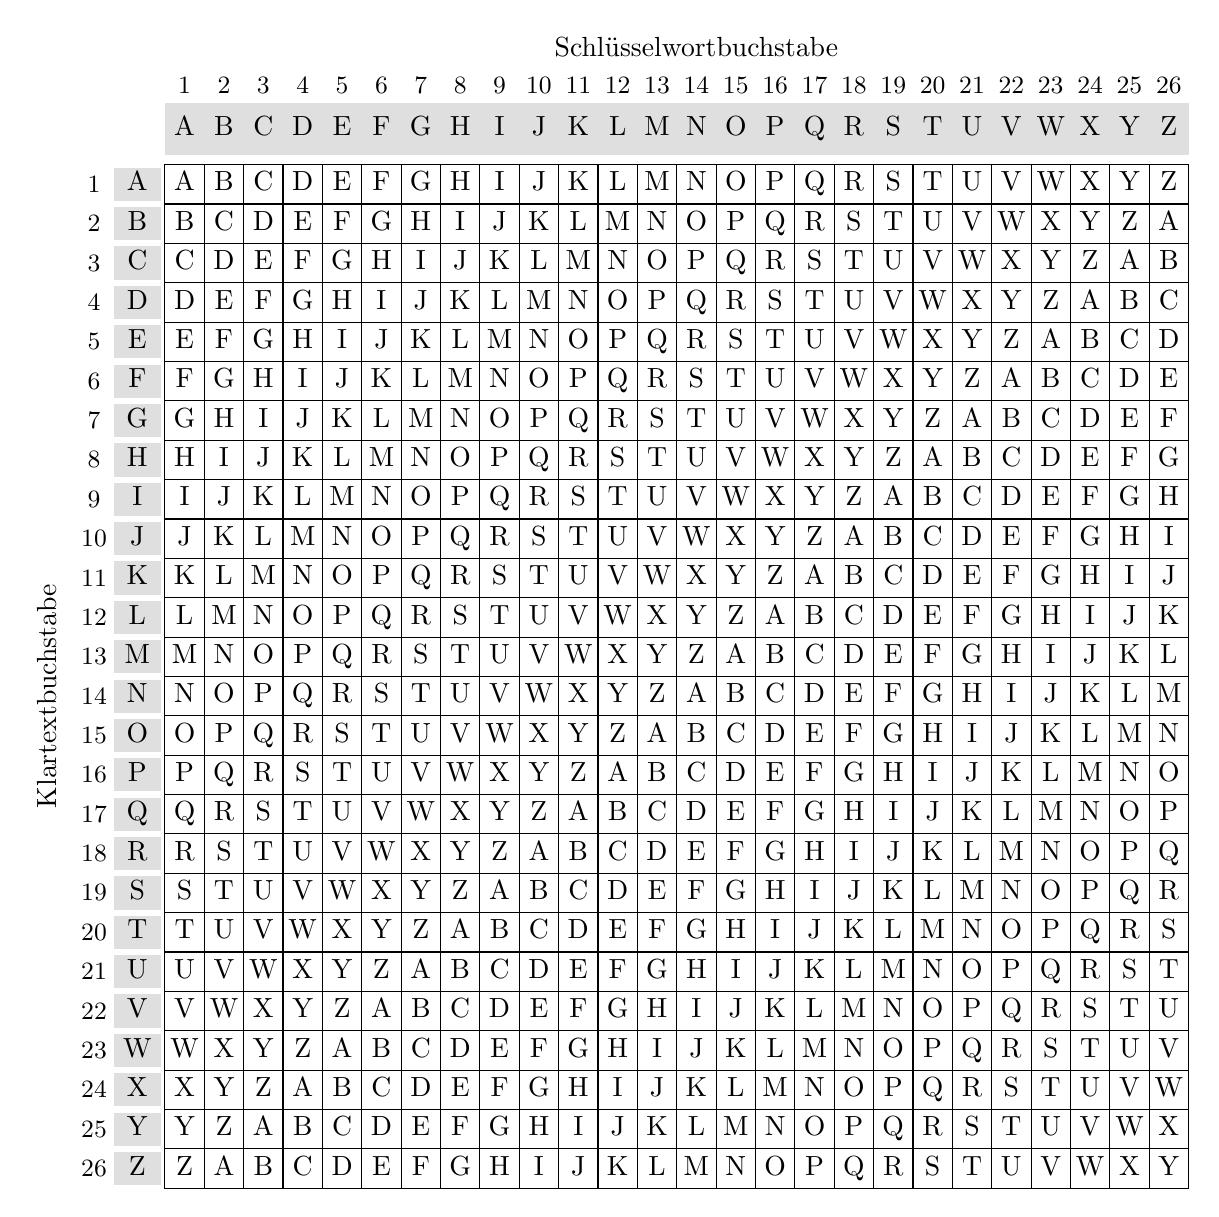
\begin{tikzpicture}
\foreach \i in {0,...,25} {
  \foreach \j in {0,...,25} {
    \edef\k{\ifnum\numexpr\i+\j\relax>25
        \the\numexpr\i+\j-26\relax
      \else
        \the\numexpr\i+\j\relax
      \fi}
 	\node[draw, minimum size=0.5cm, inner sep=0pt] at (\i*0.5,-\j*0.5) {\strut\symbol{\numexpr`A+\k\relax}};
  }
  \node[fill=gray!25, minimum width=0.6cm, inner sep=0pt, outer sep=0pt] at (-0.6,-\i*0.5) {\strut\symbol{\numexpr`A+\i\relax}};
  \node[minimum width=0.6cm] at (-1.15,-\i*0.5) {\small \the\numexpr\i+1};
  
  \node[fill=gray!25, minimum width=0.5cm] at (\i*0.5,0.7)   {\strut\symbol{\numexpr`A+\i\relax}};
  \node[minimum width=0.5cm] at (\i*0.5,1.25) {\small \the\numexpr\i+1};
}

\node[rotate=90, anchor=north] at (-2,-6.5) {Klartextbuchstabe};
\node at (6.5,1.75) {Schlüsselwortbuchstabe};
\end{tikzpicture}
\end{figure}

\fillwithgrid{\stretch{1}}

\newpage

\section{Das Kryptosystem \texttt{VIGENÈRE-ABSTRAKT}}

Wir können das Kryptosystem \texttt{VIGENÈRE} auch ohne das Vigenère-Quadrat verwenden. Dazu müssen wir jedem Buchstaben eine natürliche Zahl zuordnen. Die Verschlüsselung geschieht dann durch die modulare Addition zweier Zahlen. Die Entschlüsselung durch die modulare Subtraktion. Wir nennen dieses Kryptosystem \texttt{VIGENÈRE-ABSTRAKT}, da es ohne Vigenère-Quadrat auskommt.

\subsection{Zuordnung von Buchstaben zu Zahlen}

Wir ordnen den 26 Buchstaben jeweils eine Zahl aus $\mathbb{Z}_{26} = \{0, 1, 2, 3, \dots, 23, 24, 25\}$ zu. \autoref{table-vigenere-abstrakt} zeigt die Zuordnung.

\begin{table}[htb]
\centering
\begin{tblr}{
    colspec = {|c|c|c|c|c|c|c|c|c|c|c|c|c|}
}
\hline
A  & B  & C  & D  & E  & F  & G  & H  & I  & J  & K  & L  & M  \\ \hline
0  & 1  & 2  & 3  & 4  & 5  & 6  & 7  & 8  & 9  & 10 & 11 & 12 \\ \hline[2pt]
N  & O  & P  & Q  & R  & S  & T  & U  & V  & W  & X  & Y  & Z  \\ \hline
13 & 14 & 15 & 16 & 17 & 18 & 19 & 20 & 21 & 22 & 23 & 24 & 25 \\ \hline
\end{tblr}
\caption{Codierung ($\neq$ Verschlüsselung) der \num{26} Buchstaben.}
\label{table-vigenere-abstrakt}
\end{table}

Diese Tabelle stellt \textbf{keine} Verschlüsselung dar. Es ist eine \textbf{Codierung} und ist somit öffentlich bekannt. \textbf{Vor} der eigentlichen Verschlüsselung codieren wir den Klartext mit \autoref{table-vigenere-abstrakt}. Nach der eigentlichen Entschlüsselung erhalten wir den Kryptotext durch eine Decodierung mit \autoref{table-vigenere-abstrakt}.

\subsection{Verschlüsselung und Entschlüsselung}

Die \textbf{Verschlüsselung} erfolgt analog zu \texttt{VIGENÈRE}. Pro Buchstabe führen wir diese Schritte durch:

\begin{enumerate}
	\item \label{item-cipher-vigenere-abstrakt-1} Codiere den \textbf{Klartextbuchstaben} mit \autoref{table-vigenere-abstrakt}. Dies ist der erste Summand.
	\item \label{item-cipher-vigenere-abstrakt-2} Codiere den \textbf{Schlüsselwortbuchstaben} mit \autoref{table-vigenere-abstrakt}. Dies ist der zweite Summand.
	\item \label{item-cipher-vigenere-abstrakt-3} \textbf{Addiere} die beiden Zahlen aus \ref{item-cipher-vigenere-abstrakt-1}. (erster Summand) und \ref{item-cipher-vigenere-abstrakt-2}. (zweiter Summand) mit $\bmod 26$.
	\item Decodiere das Ergebnis aus \ref{item-cipher-vigenere-abstrakt-3}. mit \autoref{table-vigenere-abstrakt}, um den \textbf{Kryptotextbuchstaben} zu erhalten.
\end{enumerate}

\begin{example}
Wir verschlüsseln den Klartext PARTY mit dem Schlüssel KSWE.

\begin{table}[htb]
\resizebox{\textwidth}{!}{%
\begin{tblr}{
    colspec = {|Q[c, m]|Q[c, m]|Q[c, m]|Q[c, m]|Q[c, m]|Q[c, m]|Q[c, m]|Q[c, m]|Q[c, m]|Q[c, m]|Q[c, m]|Q[c, m]|}
}
\hline
Klartext   		& P & A & R & T & Y & \SetCell[r=2]{c}{$\xrightarrow{\makebox[2cm]{Codieren}}$} & 15 & 0 & 17 & 19 & 24  \\ \hline
Schlüssel  	& K & S & W & E & K &  & 10 & 18 & 22 & 4 & 10  \\ \hline
  			&  &  &  &  &  & {Modulare \\ Addition} & $15 \oplus_{26} 10$ & $0 \oplus_{26} 18$ & $17 \oplus_{26} 22$ & $19 \oplus_{26} 4$ & $24 \oplus_{26} 10$  \\ \hline[2pt]
Kryptotext 	& Z & S & N & X & I & $\xleftarrow{\makebox[2cm]{Decodieren}}$ & 25 & 18 & 13 & 23 & 8  \\ \hline
\end{tblr}
}
\end{table}
\end{example}

\begin{hinweis}
Natürlich könnten auch direkt die Zahlen den Kryptotext darstellen. Wir decodieren die Zahlen jedoch wieder in die Buchstaben, damit \texttt{VIGENÈRE-ABSTRAKT} exakt die gleichen Kryptotexte wie \texttt{VIGENÈRE} erzeugt.
\end{hinweis}

Die \textbf{Entschlüsselung} erfolgt ähnlich zur Verschlüsselung. Pro Kryptotextbuchstabe führen wir diese Schritte durch:

\begin{enumerate}
	\item \label{item-decipher-vigenere-abstrakt-1} Codiere den \textbf{Kryptotextbuchstaben} mit \autoref{table-vigenere-abstrakt}. Dies ist der Minuend.
	\item \label{item-decipher-vigenere-abstrakt-2} Codiere den \textbf{Schlüsselwortbuchstaben} mit \autoref{table-vigenere-abstrakt}. Dies ist der Subtrahend.
	\item \label{item-decipher-vigenere-abstrakt-3} \textbf{Subtrahiere} die beiden Zahlen aus \ref{item-decipher-vigenere-abstrakt-1}. (Minuend) und \ref{item-decipher-vigenere-abstrakt-2}. (Subtrahend) mit $\bmod 26$.
	\item Decodiere das Ergebnis aus \ref{item-decipher-vigenere-abstrakt-3}. mit \autoref{table-vigenere-abstrakt}, um den \textbf{Klartextbuchstaben} zu erhalten.
\end{enumerate}

\newpage

\begin{example}
Wir entschlüsseln den Kryptotext KHBIV mit dem Schlüssel KSWE.

\begin{table}[htb]
\resizebox{\textwidth}{!}{%
\begin{tblr}{
    colspec = {|Q[c, m]|Q[c, m]|Q[c, m]|Q[c, m]|Q[c, m]|Q[c, m]|Q[c, m]|Q[c, m]|Q[c, m]|Q[c, m]|Q[c, m]|Q[c, m]|}
}
\hline
Kryptotext   		& K & H & B & I & V & \SetCell[r=2]{c}{$\xrightarrow{\makebox[2cm]{Codieren}}$} & 10 & 7 & 1 & 8 & 21  \\ \hline
Schlüssel  	& K & S & W & E & K &  & 10 & 18 & 22 & 4 & 10  \\ \hline
  			&  &  &  &  &  & {Modulare \\ Subtraktion} & $10 \ominus_{26} 10$ & $7 \ominus_{26} 18$ & $1 \ominus_{26} 22$ & $8 \ominus_{26} 4$ & $21 \ominus_{26} 10$  \\ \hline[2pt]
Klartext 	& A & P & F & E & L & $\xleftarrow{\makebox[2cm]{Decodieren}}$ & 0 & 15 & 5 & 4 & 11  \\ \hline
\end{tblr}
}
\end{table}
\end{example}

Wir haben mit \texttt{VIGENÈRE-ABSTRAKT} erneut für ein Kryptosystem die \textbf{Darstellung} verändert. Die Eigenschaften und insbesondere die Sicherheit des Kryptosystems \texttt{VIGENÈRE-ABSTRAKT} ist \textbf{identisch} zum Kryptosystem \texttt{VIGENÈRE}. Warum haben wir diesen Aufwand betrieben? Wir haben nun gesehen, dass ein Kryptosystem allein durch \textbf{mathematische Operationen} dargestellt werden kann. Dies erleichtert den Einbau in ein \textbf{Computerprogramm} deutlich. Praktisch alle modernen Kryptosysteme basieren auf mathematischen Operationen.

\subsection{Aufgaben}

Bei allen Aufgaben ist das Kryptosystem \texttt{VIGENÈRE-ABSTRAKT} zu verwenden. Notieren Sie \textbf{alle} Zwischenschritte.

\begin{enumerate}
\item Verschlüsseln Sie CAMPUS. Verwenden Sie COLA als Schlüssel.

\fillwithgrid{2in}

\item Verschlüsseln Sie WETTINGEN. Verwenden Sie STERN als Schlüssel.

\fillwithgrid{\stretch{1}}

\newpage

\item Entschlüsseln Sie USZRVTFGL. Verwenden Sie CDREIPO als Schlüssel.

\fillwithgrid{2.5in}

\item Entschlüsseln Sie UZNXPYZZIZ. Verwenden Sie RZWEIDZWEI als Schlüssel.

\fillwithgrid{2.5in}

\item Der Klartext lautet 17 8 21 4 17 18 8 3 4. Der Kryptotext lautet 6 16 20 3 17 7 16 2 3. \textbf{Berechnen} Sie den Schlüssel und \textbf{decodieren} Sie dann das Ergebnis.

\fillwithgrid{\stretch{1}}

\end{enumerate}

